\documentclass{article}
\usepackage[top=10mm, bottom=10mm]{geometry}
\usepackage{amsmath}
\usepackage{graphicx}
\usepackage{circuitikz}
\usepackage{float}

\let\vec\mathbf
\newcommand{\myvec}[1]{\ensuremath{\begin{pmatrix}#1\end{pmatrix}}}

\title{Hardware Assignment}
\author{AI25BTECH11023 - Pratik Raj\\
AI25BTECH11035 - Sujal Rajani}
\date{}

\begin{document}
\maketitle

\section{Introduction}

This report details the process of determining the voltage across a 
PT-100 RTD (Resistance Temperature Detector) as a function of temperature.
The least squares method was used to estimate the parameters of the
Callendar-Van Dusen equation.

\section{Collecting Data}

We were provided with the following components
\begin{itemize}
    \item PT-100 Resistance Temperature Detector
    \item Arduino Uno and USB Cable
    \item 10 $\Omega$ resistor
    \item Breadboard
    \item Wires
\end{itemize}

We also made use of the following items from the EE Lab to
control and monitor the temperature
\begin{itemize}
    \item Electric kettle
    \item Digital Thermometer
\end{itemize}

The 100 $\Omega$ resistor and the PT-100 were connected in series
between the 5V output pin and the ground pin of the Arduino to create
a voltage divider. The other pin of the PT-100 is connected to the
A0 pin of the Arduino to measure the voltage across the PT-100.

\begin{figure}[h!]
    \centering
    \begin{circuitikz} \draw
        (0,0) to[battery1, l=$5\ V$, invert] (0,2)
        to[R, l^=$10\ \Omega$] (3,2) to[short, -o] (5,2) node[right] {A0 (Arduino)};
        \draw (3,2) to[R, l^=$P\ \Omega$ (PT-100)] (3,0)
        -- (0,0);
        \draw (3,0) to[short, -o] (5,0) node[right] {GND (Arduino)};
    \end{circuitikz}
\end{figure}

The PT-100 was immersed in an electric kettle filled with water, and a digital
thermometer was used to measure the temperature.

The kettle was turned on for some time, and then turned off. Once the reading of
the digital thermometer becaome stable, a reading was taken, and the Temperature
was increased again. A total of 30 readings were taken over a range of temperatures
from 26.8 $^\circ$C to 97.8 $^\circ$C.

17 points were randomly chosen from the data set to form the
training set. The remaining 13 points were put in the
testing set.

\begin{figure}
    \centering
    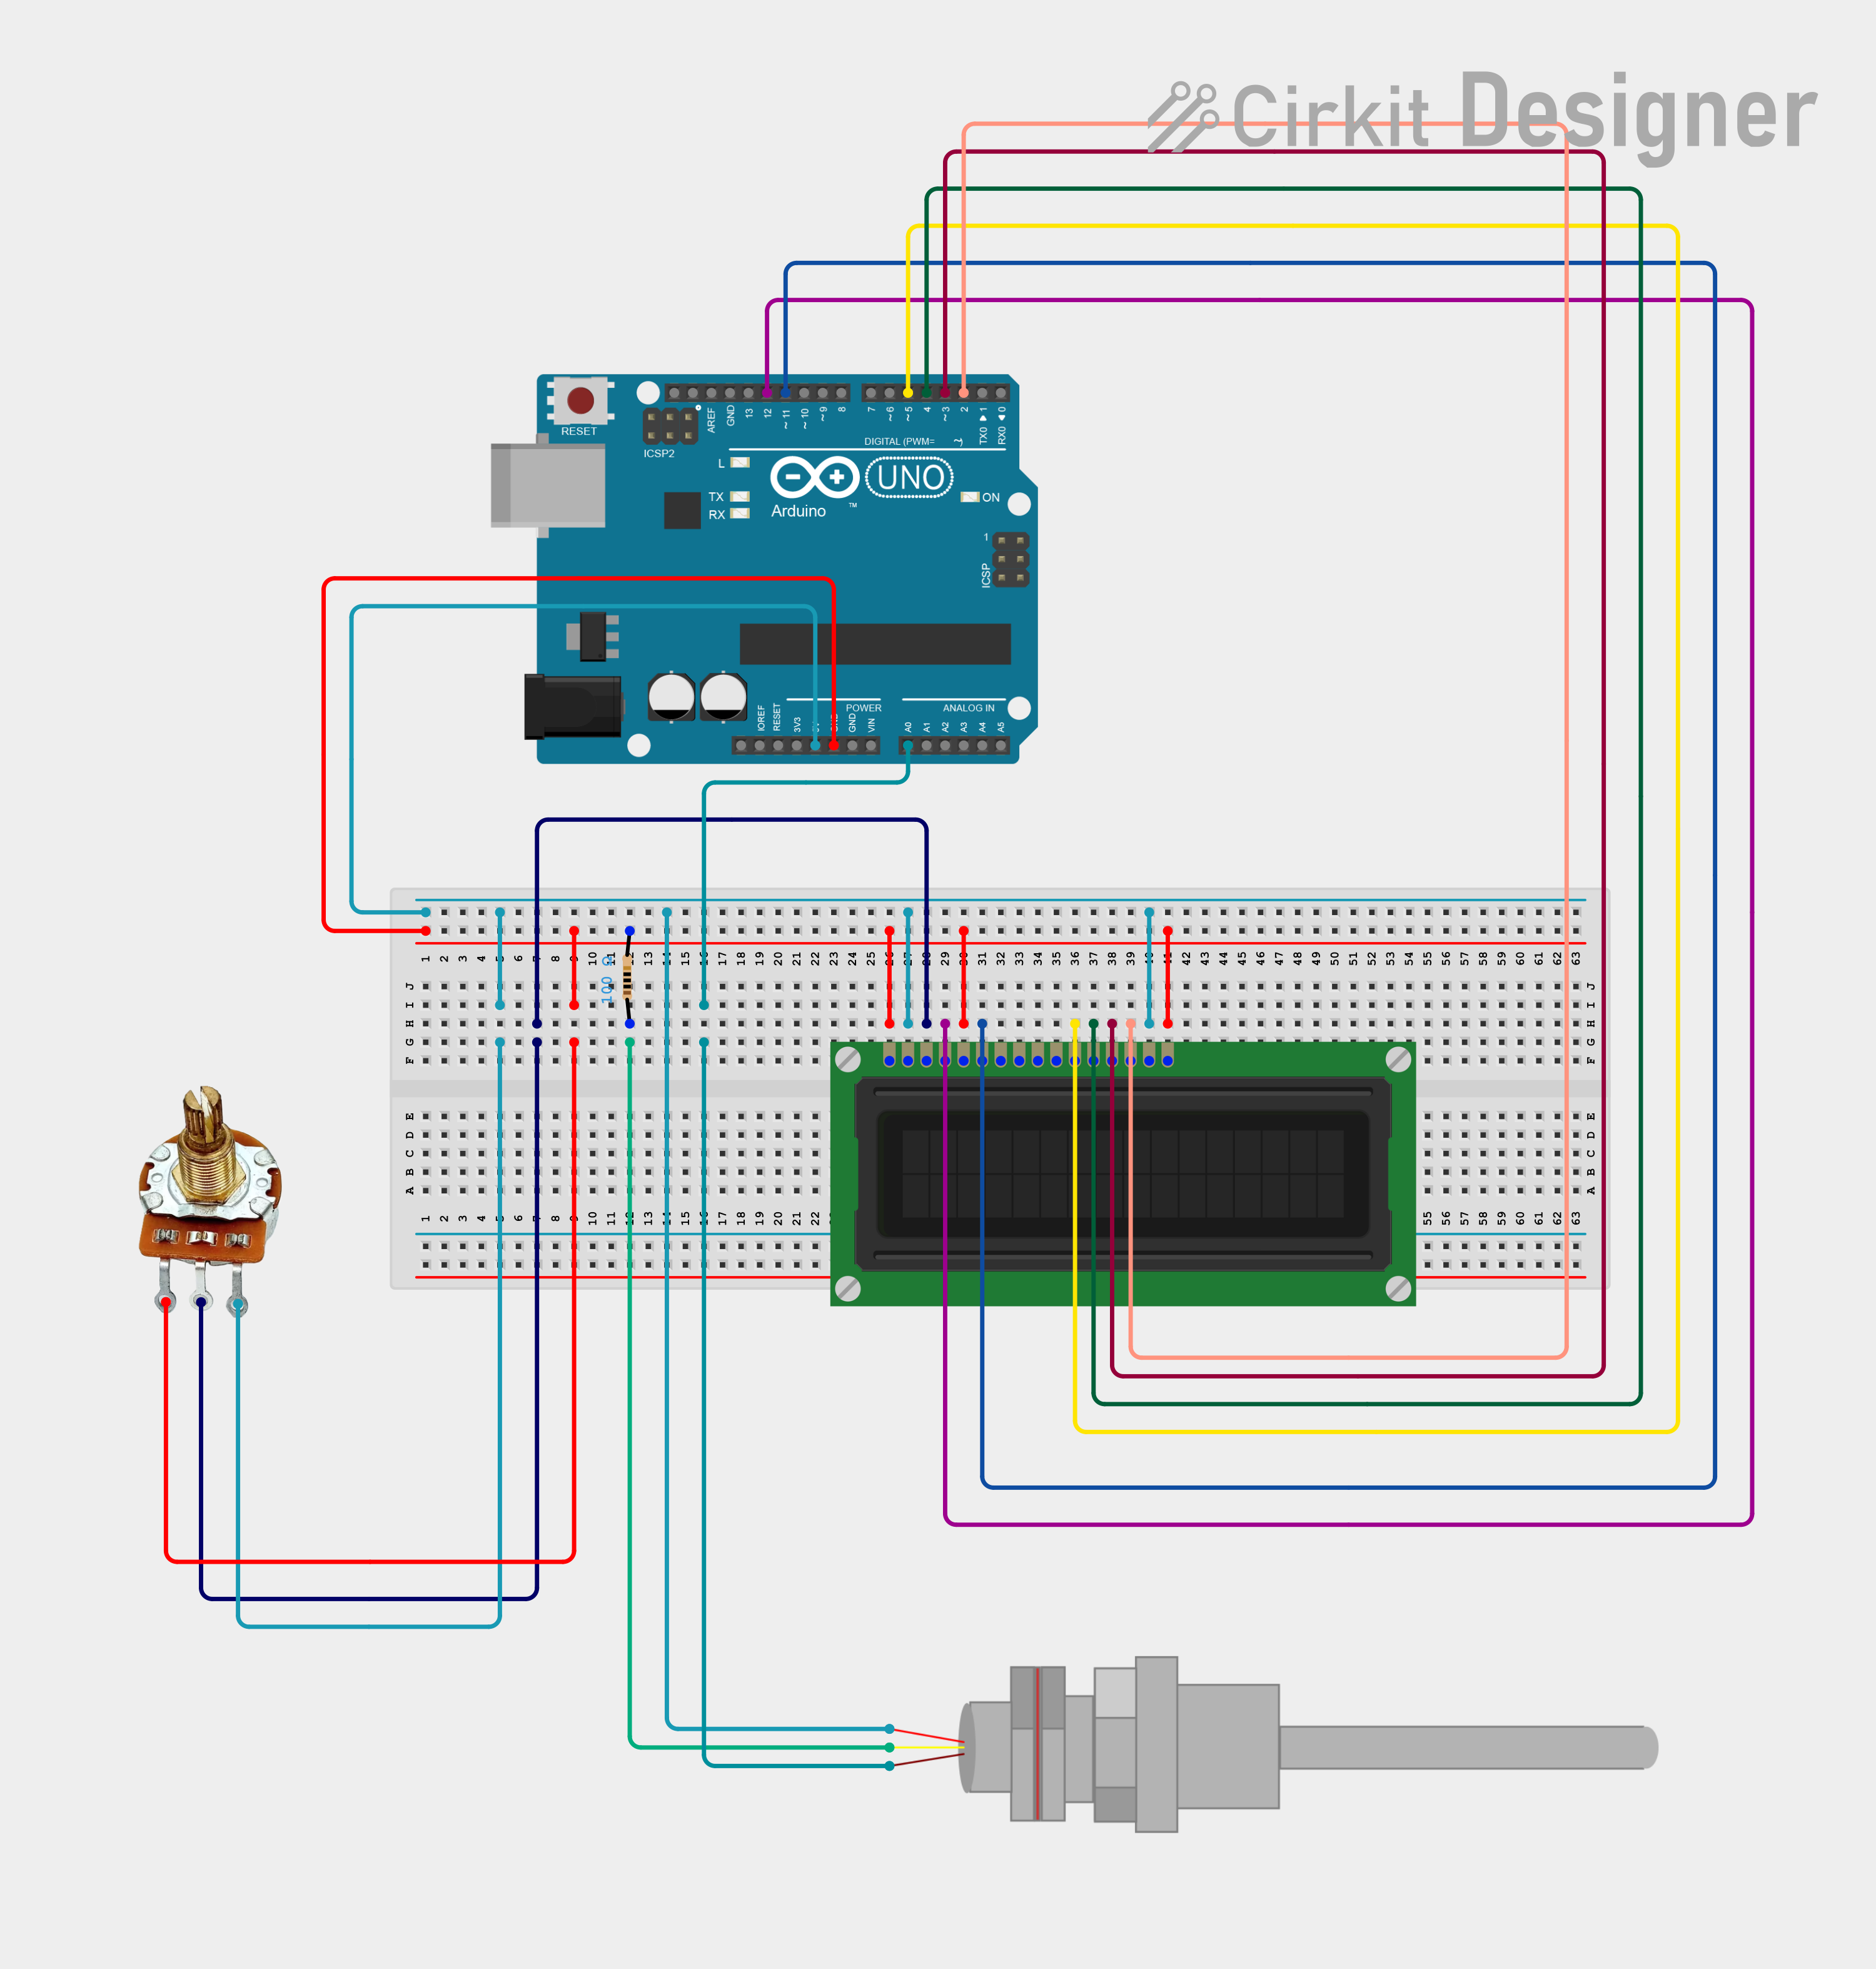
\includegraphics[width=1\linewidth]{figs/circuit_image.png}
    \caption{Circuit Diagram}
    \label{fig:placeholder}
\end{figure}
\newpage
\section{Model}

We use the Callendar-Van Dusen equation to model the voltage across the PT-100
as a quadratic function of temperature.

\begin{align}
    V(T) &= n_0 + n_1T + n_2T^2 \\
    c &= \vec{n}^\top \vec{x} \\
\end{align}

where

\begin{align}    
    c &= V(T), \vec{n} = \myvec{n_0 \\ n_1 \\ n_2}, \vec{x} = \myvec{1 \\ T \\ T^2}
\end{align}

We can write the equation in matrix form as

\begin{align}
    \vec{X}^\top \vec{n} = \vec{C}
\end{align}

where

\begin{align}
    \vec{X} = \myvec{1 & 1 & \dots & 1 \\ T_1 & T_2 & \dots & T_n \\ T_1^2 & T_2^2 & \dots & T_n^2},
    \vec{C} = \myvec{V(T_1) \\ V(T_2) \\ \vdots \\ V(T_n)}
\end{align}

Using Least Square Method

\begin{align}
\vec{n} = \brak(\vec{X} \vec{X}^\top)^{-1} \vec{X} \vec{C}
\end{align}

For the $PT-100$ data, the approximate model is given by


\begin{align}
    V(T) = 2.23689 + 0.00130T + (-3.07 \times 10^{-5})T^2
\end{align}

\begin{align}
    \vec{n} = \myvec{2.23689\\ 0.00130 \\ -3.07 \times 10^{-5}}
\end{align}
\begin{table}
\caption{Temperature and Voltage Data}
\label{tab:temp_voltage}
\begin{tabular}{r|r}

Temperature & Voltage \\

26.800000 & 2.270000  \\
38.000000 & 2.228700 \\
42.500000 & 2.250000  \\
48.900000 & 2.240000 \\
54.500000 & 2.210000 \\
37.100000 & 2.228700  \\
79.100000 & 2.150000 \\
85.000000 & 2.130000 \\
91.600000 & 2.100000 \\
94.100000 & 2.080000  \\
97.800000 & 2.070000  \\
33.300000 & 2.230000  \\
66.100000 & 2.200000  \\
76.800000 & 2.170000 \\
81.100000 & 2.140000 \\
73.800000 & 2.150500 \\
69.600000 & 2.170100  \\

\end{tabular}
\end{table}
\begin{figure}
    \centering
    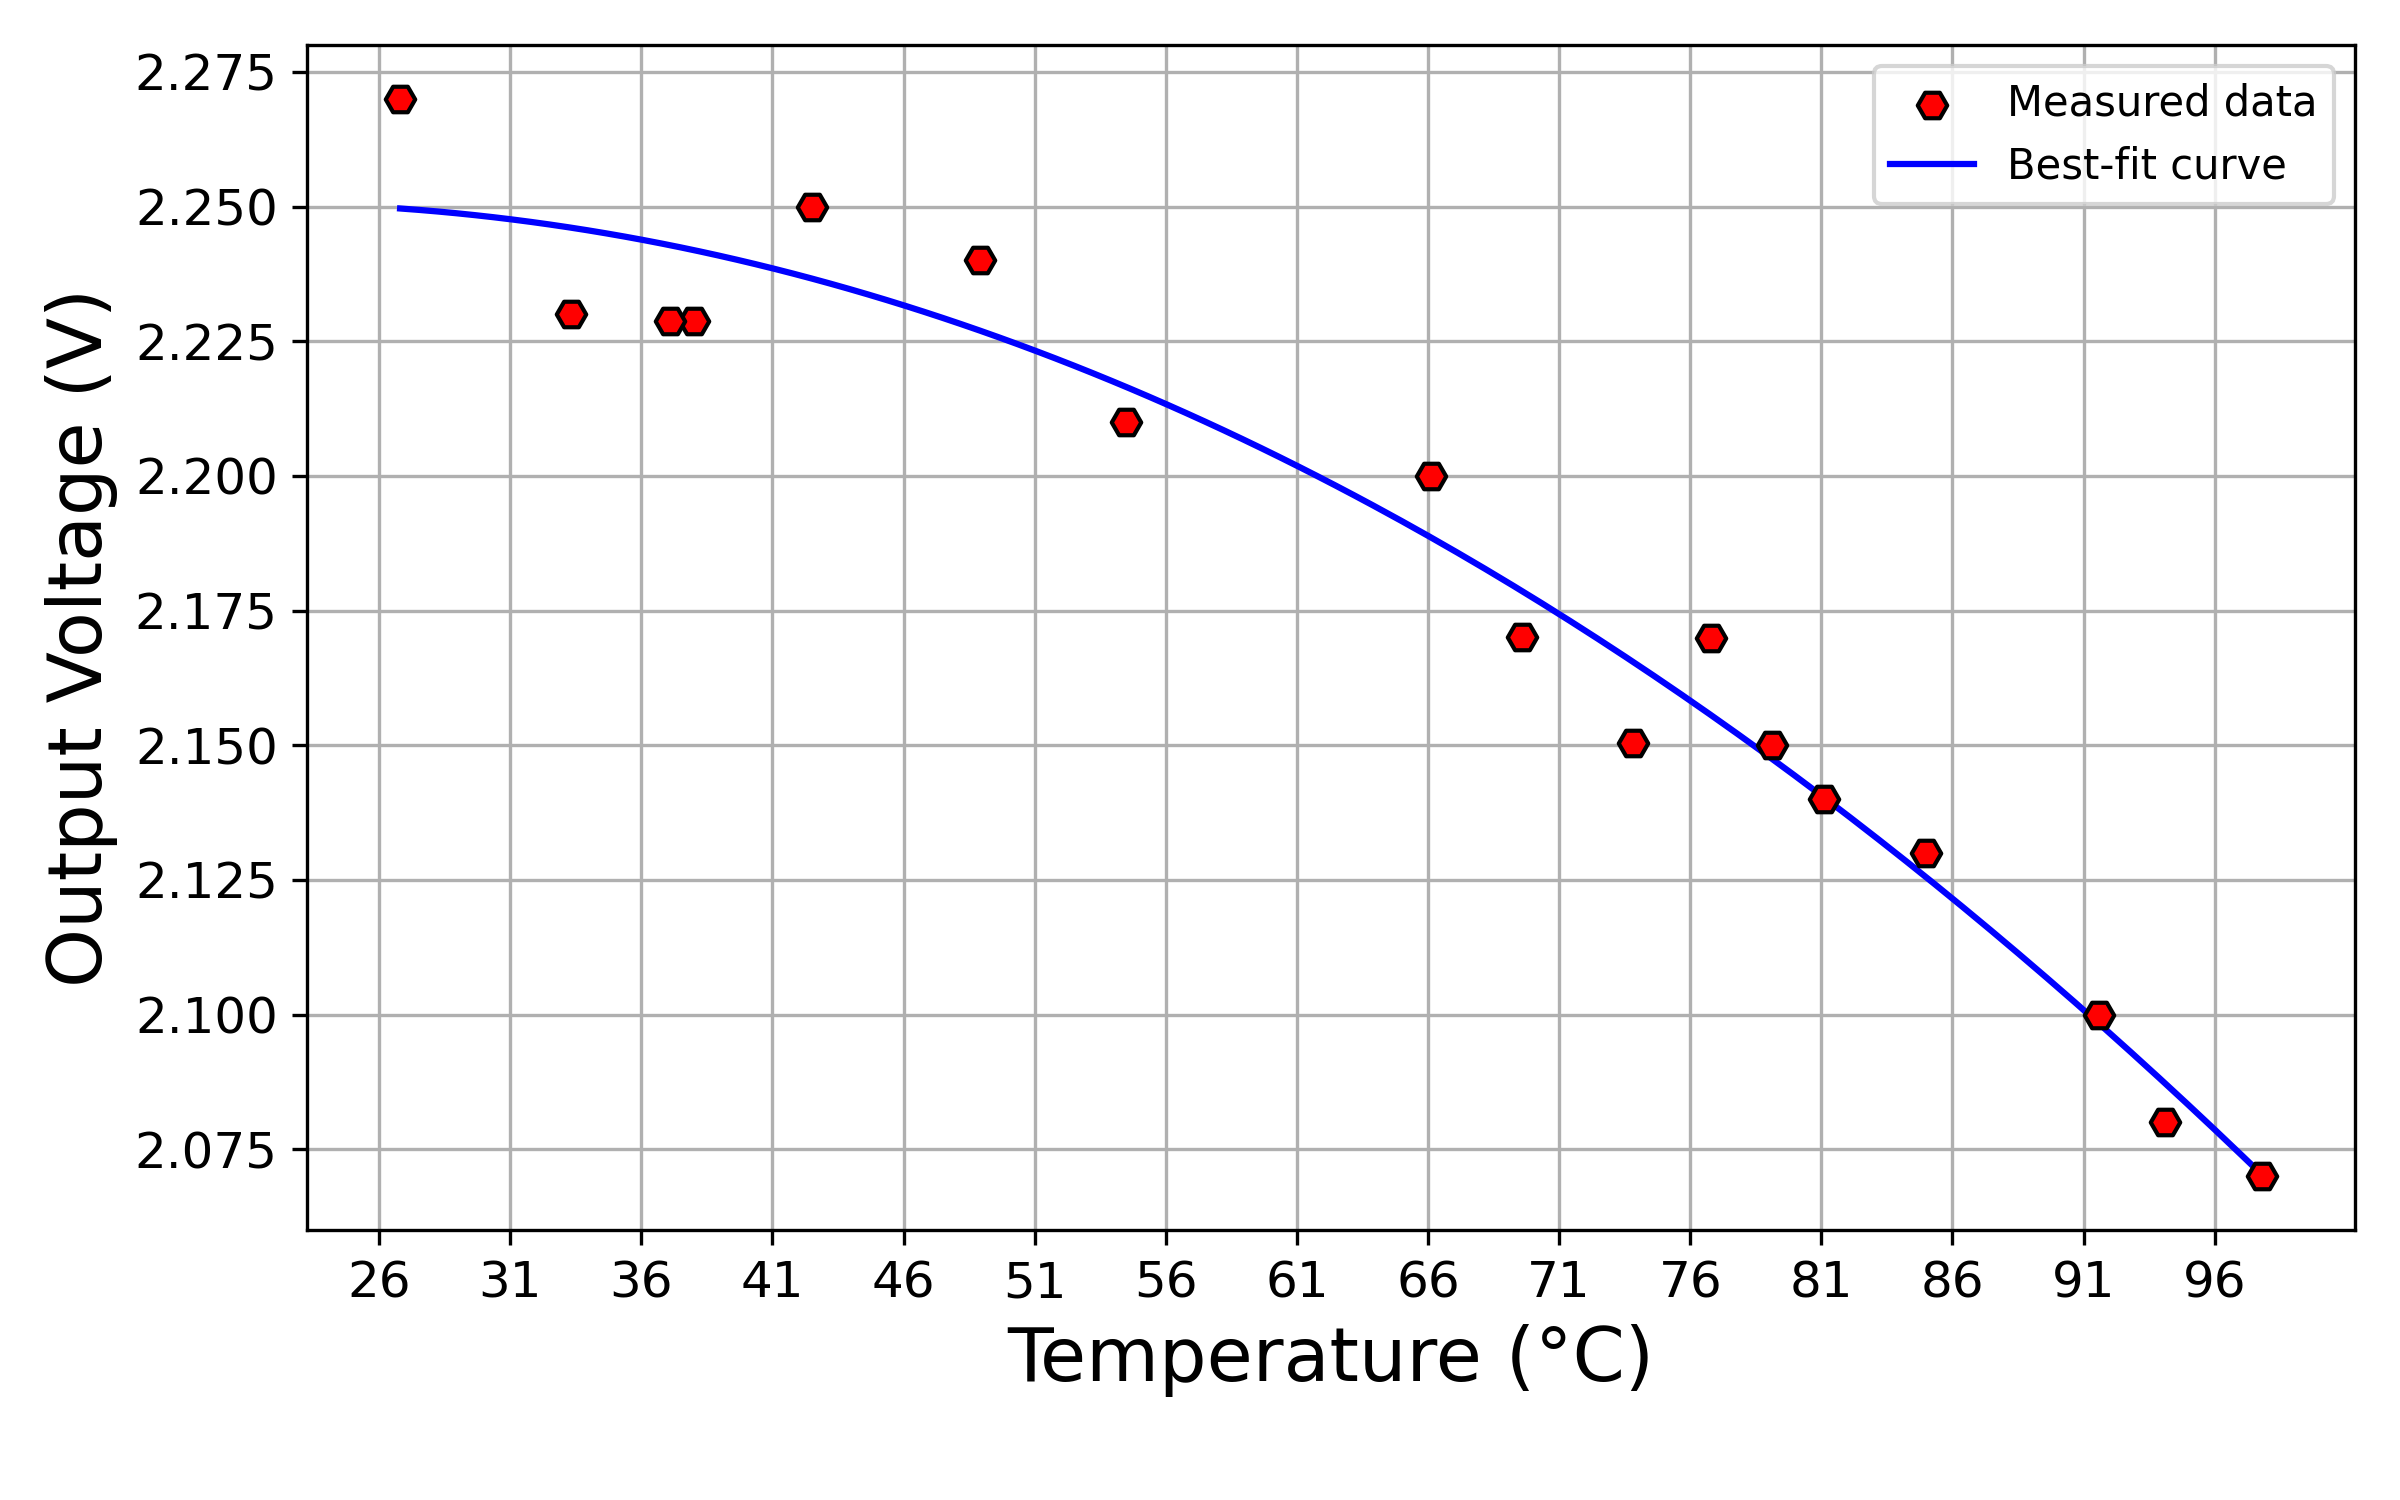
\includegraphics[width=1\linewidth]{figs/train.png}
    \caption{Training regression model}
    \label{fig:placeholder}
\end{figure}
\newpage
To  obtain temperature as a function of voltage, we rearrange or numerically invert the above equation 

\begin{align}
    T(V) = a_0 + a_1V + a_2V^2
\end{align}

The coefficients can be again found by applying the least square method to given data
\begin{align}
\myvec{1 & 1 & ... & 1\\
V_1 & V_2 & ... & V_n\\
(V_1)^2 & (V_2)^2 & ... & (V_n)^2}^\top  \myvec{a_0\\a_1\\a_2} = \myvec{T_1\\T_2\\.\\.\\.\\T_n}
\end{align}

we get
\begin{align}
\myvec{a_0\\a_1\\a_2} = \myvec{-3460.32\\3619.11\\-917.98}
\end{align}
\begin{align}
    T(V) = -3460.32 + 3619.11V + -917.98V^2
\end{align}
To obtain the temperature, we will use the above equation

\section{Validation}
The model can be validated by using test dataset

\documentclass{article}
\usepackage{graphicx}
\usepackage{booktabs}

\begin{document}

\section*{Validating the Model using Test Data}

\begin{table}[h!]
\centering
\begin{tabular}{|c|c|c|}
\hline
\textbf{Voltage (V)} & \textbf{Actual Temperature (°C)} & \textbf{Measured Temperature (°C)} \\
\midrule
1.79 & 61.2 & 62.99 \\ \hline
1.98 & 59.6 & 61.58 \\  \hline
1.57 & 58.6 & 60.17 \\  \hline 
1.55 & 50.6 & 49.05 \\  \hline
1.92 & 49.6 & 47.68 \\  \hline
1.57 & 75.8 & 77.37 \\  \hline
1.50 & 78.8 & 80.30 \\  \hline
1.57 & 80.2 & 81.77 \\  \hline
1.93 & 84.6 & 86.53 \\  \hline
1.22 & 83.9 & 85.12 \\  \hline
0.94 & 55.6 & 56.54 \\  \hline
0.85 & 46.9 & 46.05 \\  \hline
0.86 & 57.9 & 58.76 \\  \hline
0.78 & 51.2 & 50.42 \\  \hline
0.82 & 48.7 & 49.52 \\  \hline
0.72 & 84.4 & 85.12 \\  \hline
1.22 & 82.5 & 83.72 \\  \hline
0.87 & 80.9 & 81.77 \\  \hline
\end{tabular}
\caption{Validation Table}
\label{tab:temp_voltage}
\end{table}

\end{document}

\newpage
\begin{figure}
    \centering
    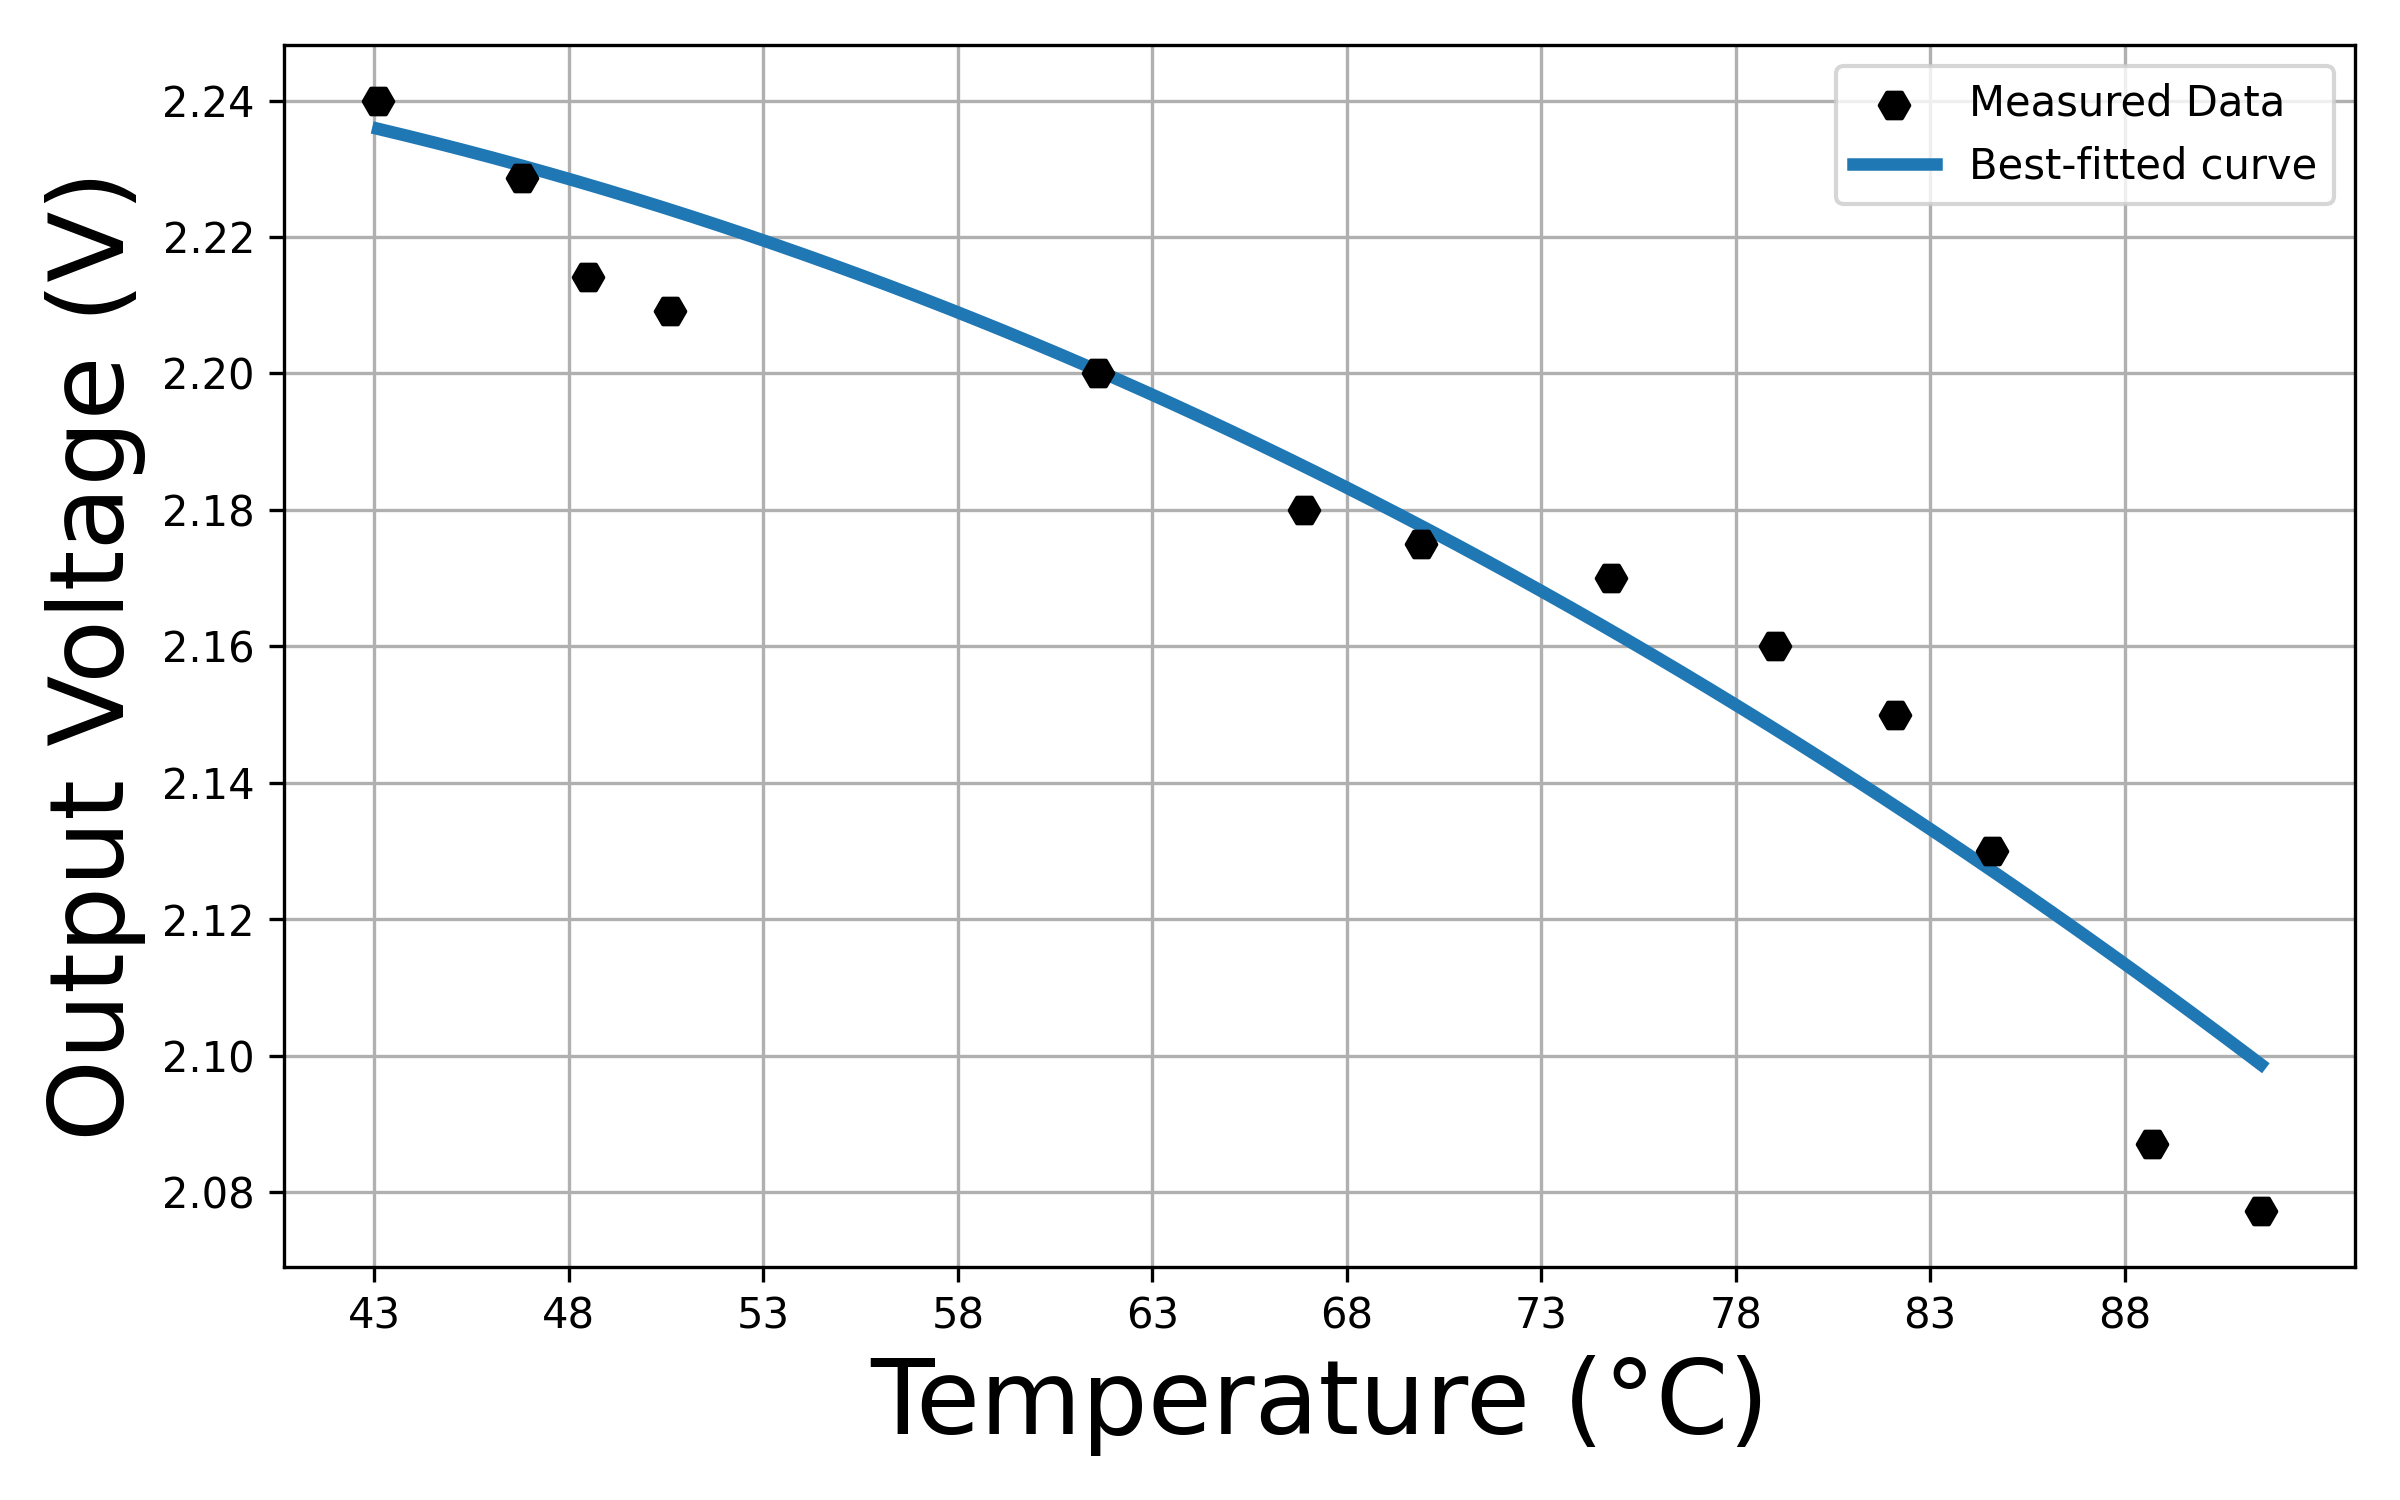
\includegraphics[width=1\linewidth]{figs/test.png}
    \caption{testing the trained model}
    \label{fig:placeholder}
\end{figure}

\section{Error \& Conclusion}
Calculating error by Mean Absolute Error (MAE)

\begin{align}
    MAE = \frac{\Sigma |T_{PT-100}-T_{A_i}|}{13}
\end{align}
where 

$T_{PT-100}$ is Temperature from PT-100 Model

$T_A$ is Actual Temperature reading

we get 
\begin{align}
MAE = 3.58 ^\circ C
\end{align}

The model produces an error of $3.58^\circ$C, demonstrating reliable predictive accuracy for the system.

\subsection*{Source of error may be:}

\begin{enumerate}
    \item Measurement noise in voltage reading
    \item Non-linearity in the PT-100 response
    \item Approximation errors in the least square method
    \item Temperature sensor calibration uncertainties
\end{enumerate}

The PT-100 sensor, when integrated with machine learning calibration, provided consistent and interpretable results suitable for practical applications.
\end{document}